\documentclass{report}

\usepackage{graphicx}

\title{Lets write the most awesome book ever!}
\author{Hasan Ali Khattak}



\begin{document}
\maketitle

\section*{Introduction}
This chapter tells the story of a very strange person. Always looking for adventures, however, he never came across anything unusual. So, he was bored in life most of the time.

\subsection{Details}
\subsubsection{Age}
His age is $ a - 1980$, here $a$ is today. which is the year in which the Einstein's equation was published, probably. %I, am not sure
The Equation says that every mass can be almost converted to energy with the use of Equation \ref{eq1}

\begin{equation}\label{eq1}
    e = m c^2
\end{equation}

\subsection{Getting out of boredom}
With the passage of time, he realized that life doesnt always give you adventures. Rather, one needs to find adventures in everyday routines.

\begin{figure}[pb]
    \centering
    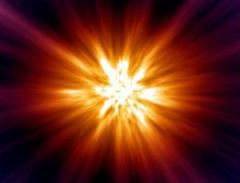
\includegraphics[width=0.5\linewidth]{figs/bigBangPicture.png}
    \caption{The moment of knowlegde explosion depicted as a big bang event.}
    \label{fig1:bigBangPicture}
\end{figure}

\subsection{Eureka}
This made him realize that everything he was doing was fun and he had been living a life full of adventures. This indeed was a moment of knowledge explosion, almost similar to him a big band. You know big bang, right ! Figure \ref{fig1:bigBangPicture}

\end{document}